\chapter{Introducción al cálculo vectorial $\; \divideontimes$}

\textcolor{gris}{ El estudio de los vectores se origina con la invención de los cuaterniones de Hamilton, quien junto a otros los desarrollaron como herramienta matemáticas para la exploración del espacio físico. Pero los resultados fueron desilusionantes, porque vieron que los cuaterniones eran demasiado complicados para entenderlos con rapidez y aplicarlos fácilmente.}

\textcolor{gris}{ Los cuaterniones contenían una parte escalar y una parte vectorial, y las dificultades surgían cuando estas partes se manejaban al mismo tiempo. Los científicos se dieron cuenta de que muchos problemas se podían manejar considerando la parte vectorial por separado y así comenzó el Análisis Vectorial.}

\textcolor{gris}{ Este trabajo se debe principalmente al físico estadounidense Josiah Willard Gibbs (1839-1903) y al físico matemático inglés Oliver Heaviside (1850-1925)}


\textcolor{gris}{ El cálculo vectorial, análisis vectorial o cálculo multivariable es un campo de las matemáticas referidas al análisis real multivariable de vectores en 2 o más dimensiones. Es un enfoque de la geometría diferencial como conjunto de fórmulas y técnicas para solucionar problemas muy útiles para la ingeniería y la física. Consideramos los campos vectoriales, que asocian un vector a cada punto en el espacio, y campos escalares, que asocian un escalar a cada punto en el espacio. Por ejemplo, la temperatura de una piscina es un campo escalar: a cada punto asociamos un valor escalar de temperatura. El flujo del agua en la misma piscina es un campo vectorial: a cada punto asociamos un vector de velocidad.} 

\textcolor{gris}{ Cuatro operaciones son importantes en el cálculo vectorial: }

\textcolor{gris}{ •	Gradiente: mide la tasa y la dirección del cambio en un campo escalar; el gradiente de un campo escalar es un campo vectorial.}

\textcolor{gris}{ •	Rotor o rotacional: mide la tendencia de un campo vectorial a rotar alrededor de un punto; el rotor de un campo vectorial es otro campo vectorial.}

\textcolor{gris}{ •	Divergencia: mide la tendencia de un campo vectorial a originarse o converger hacia ciertos puntos; la divergencia de un campo vectorial es un campo escalar.}

\textcolor{gris}{ •	Laplaciano: relaciona el "promedio" de una propiedad en un punto del espacio con otra magnitud, es un operador diferencial de segundo orden.}

\textcolor{gris}{ La mayoría de los resultados analíticos se entienden más fácilmente usando la maquinaria de la geometría diferencial, de la cual el cálculo vectorial forma un subconjunto.}

\rightline{\textcolor{gris}{Fuente: Wikipedia}}

\begin{figure}[H]
	\centering
	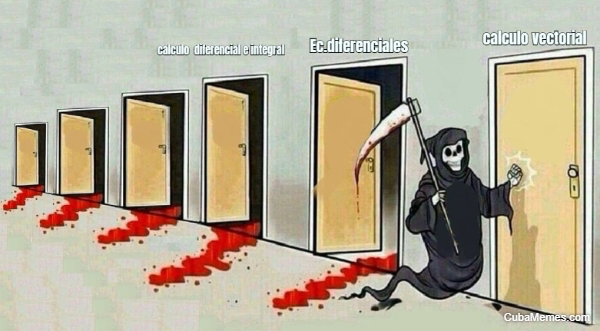
\includegraphics[width=1\textwidth]{imagenes/imagenes10/xisteCalcVect.png}
\end{figure}

\section{Resumen de la geometría vectorial aprendida hasta ahora}


\subsection{Vectores en el espacio ($\mathbb R^3$)}

$\vec v= \overrightarrow { AB }  $: segmento orientado. Origen A y extremo B
	\begin{multicols}{2}		
	\begin{itemize}
	\item \textit{módulo}: $|\vec v|=d(A,B)$
	\item \textit{dirección}: la de la recta $r$ y la de todas las paralelas a $r$
	\item \textit{sentido}: desde $A$ hacia $B$
	\end{itemize}
	\begin{figure}[H]
		\centering
		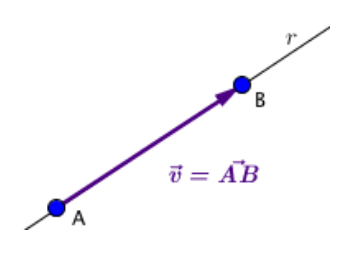
\includegraphics[width=0.4\textwidth]{imagenes/imagenes10/T10IM01.png}
	\end{figure}
	\end{multicols}

Vectores LIBRES, se pueden trasladar paralelamente a sí mismos por todo el espacio.
				
Dos vectores son IGUALES si tienen el mismo módulo, la misma dirección y el mismo sentido.

\subsection{Producto de un vector por un número real (escalar)}

$k \in \mathbb{R}$: $\ \ k\cdot \vec v$
\begin{multicols}{2}				
\begin{itemize}
	\item \textit{módulo}: $|k|\cdot |\vec v|$
	\vspace{-2mm}\item \textit{dirección}: la misma que $\vec v$
	\vspace{-2mm}\item \textit{sentido}: si $k>0$ mismo que $\vec v$; si $k<0$ contrario a $\vec v$
\end{itemize} 
\begin{figure}[H]
		\centering
		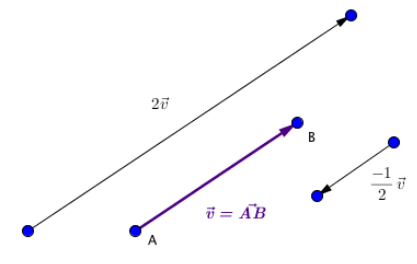
\includegraphics[width=0.3\textwidth]{imagenes/imagenes10/T10IM02.png}
\end{figure}
\end{multicols}


Dado un vector $\vec v$, un vector UNITARIO en la misma dirección que $\vec v$ se puede obtener como: $\dfrac 1 {|\vec v|}\cdot \vec v$

\vspace{4mm}

\underline{Propiedades:} 

\begin{itemize}
\begin{multicols}{2}
	\item $a\cdot (b\cdot \vec v)=(a\cdot b)\cdot \vec v$ 
	\item  $a\cdot (b\cdot \vec v)=(a\cdot b)\cdot \vec v$ 
	\item $(a+b)\cdot \vec v=a\cdot \vec v+ b\cdot \vec v  $
	\item $1\cdot \vec v=\vec v$
\end{multicols}
\end{itemize}

\subsection{Suma de vectores}

	$\vec u \pm \vec v$  (gráficamente: en matemáticas se usa la técnica de vectores concurrentes, en física es más usual el método del paralelogramo).
	\begin{multicols}{2}
	
	\begin{itemize}
		\item $(\vec u + \vec v)+ \vec w=\vec u+(\vec v + \vec w)$
		\vspace{-2mm}\item $\vec u + \vec v= \vec v+ \vec u$
		\vspace{-2mm}\item $\vec u+ \vec 0=\vec u$
		\vspace{-2mm}\item $\vec u+ (\overrightarrow {-u})=\vec 0$
	\end{itemize}
	\begin{figure}[H]
		\centering
		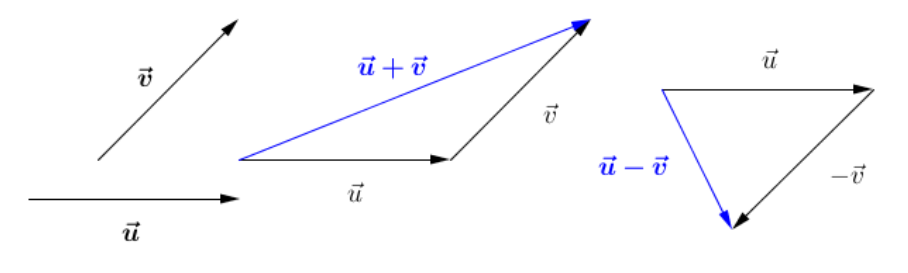
\includegraphics[width=0.5\textwidth]{imagenes/imagenes10/T10IM03.png}
	\end{figure}
	\end{multicols}
	Restar vectores = sumar el opuesto : $\vec u - \vec v = \vec u +(-\vec v)$

\begin{multicols}{2}
	\scriptsize{Puesto que los vectores con que tratamos son libres, el `método del paralelogramo' usado en física consiste en colocar los vectores unidos por sus orígenes y, mediante paralelas a éstos, construir un paralelogramo. El vector que va desde la unión de los vectores al punto opuesto de la diagonal es el vector suma}  \normalsize{:}

	\begin{figure}[H]
	\centering
	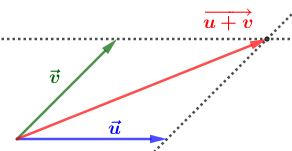
\includegraphics[width=0.3\textwidth]{imagenes/imagenes10/T10IM14.png}
	\end{figure}
\end{multicols}

\begin{multicols}{2}
	\begin{figure}[H]
	\centering
	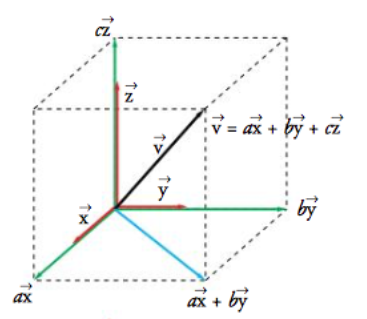
\includegraphics[width=0.30\textwidth]{imagenes/imagenes10/T10IM04.png}
	\end{figure}
	
	La suma de tres vectores de distinta dirección y no coplanarios en el espacio: 
	
	\centerline{$\vec u+\vec v+\vec w$} 
	
	es la diagonal del paralelepípedo.
\end{multicols}

\subsection{Combinación lineal de vectores}

	Dados varios vectores $\vec u_1$, $\vec u_2$, $\vec u_3$, ..., $\vec u_n$ y otros tantos números reales $\alpha_1$, $\alpha_2$, $\alpha_3$, ..., $\alpha_n$, a la expresión $\alpha_1 \vec u_1+\alpha_2 \vec u_2+\alpha_3 \vec u_3+...+\alpha_n \vec u_n$ se le llama `Combinación Lineal' de los n-vectores iniciales.
		
	%\vspace{3mm}
		
	Varios vectores se dice que son `Linealmente Dependientes'  si alguno de ellos se puede poner como combinación lineal de los demás. Si no es así, se dice que son `Linealmente Independientes'.
	

\subsection{Base}

\begin{multicols}{2}
	3 vectores cualesquiera del espacio, no coplanarios, y de direcciones distintas, $\vec x,\ \vec y, \ \vec z$ son linealmente independientes, además, cualquier otro vector del espacio se puede escribir como combinación lineal de estos tres vectores de forma única. Se dice que estos tres vectores forman una BASE $B=\{\vec x,\ \vec y, \ \vec z\}$
	\begin{figure}[H]
	\centering
	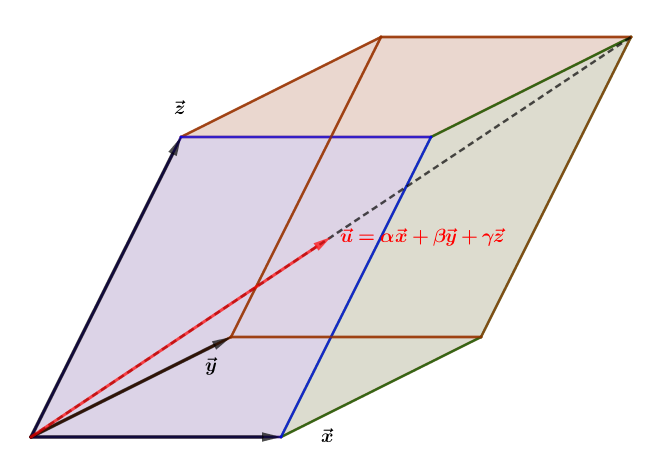
\includegraphics[width=0.40\textwidth]{imagenes/imagenes10/T10IM06.png}
	\end{figure}
\end{multicols}

\vspace{3mm}

\begin{multicols}{2}
	\begin{figure}[H]
	\centering
	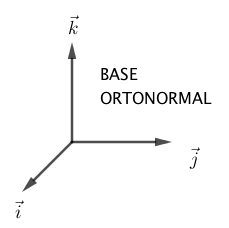
\includegraphics[width=0.30\textwidth]{imagenes/imagenes10/T10IM05.png}
	\end{figure}
	Si los vectores de la base son mutuamente perpendiculares (ortonormales) y tienen módulo 1 (unitarios), la base $B=\{\vec i, \vec j, \vec k \}$ se llama `Base OrtoNormal (BON)' 
	\footnotesize{(Orto por ortogonal, es decir, perpendiculares entre sí, y Normal porque los vectores básicos tiene norma o módulo $1$, están normalizados)}\normalsize{.}
\end{multicols}

\subsection{Operaciones con vectores dados por sus componentes}

Como cualquier vector $\vec v$  se puede expresar de forma única en cada base $B=\{\vec x,\ \vec y, \ \vec z\} \quad \to \quad \vec v= \alpha \vec x+ \beta \vec y+ \gamma \vec z$. A los parámetros de esta combinación lineal, $\alpha, \ \beta, \ \gamma$ se les llama \underline{componentes} de $\vec v$ en la base $B$, $\ \vec v=(\alpha, \ \beta, \ \gamma)$
		
Las componentes de $\vec i, \ \vec j, \ \vec k$ en la base ortonormal $B=\{ \vec i, \vec j, \vec k \} $ son $\vec i=(1,0,0); \ \vec j=(0,1,0); \ \vec k=(0,0,1)$
		
 En el espacio, los \underline{puntos} se representan por \underline{coordenadas}, $A(x_0, y_0, z_0)$ y los \underline{vectores} por \underline{componentes} $\vec u=(u_x, u_y, u_z)$


		
\vspace{3mm} $ \alpha , \ \beta \ \in \mathbb{R}; \ \vec u=(u_x,u_y,u_z); \ \vec v = (v_x ,v_y ,v_z) \to $
		
\vspace{2mm}\hspace{20mm}$\alpha \vec u+\beta \vec v=
			(\alpha  u_x+\beta  v_x,\;  \alpha  u_y+\beta  v_y,\;  \alpha  u_z+\beta  v_z) $
			
\subsection{Producto `Escalar'}

\begin{equation}
	\boxed{\ \vec u \cdot \vec v = |\vec u| \cdot |\vec v| \cdot \cos \theta \ } \ ,\ \in \mathbb{R} 
\end{equation}			

\vspace{3mm}

\begin{multicols}{2}
Geométricamente:

\emph{El producto escalar de dos vectores es el módulo de uno de ellos por la proyección del otro sobre él}
\begin{figure}[H]
	\centering
	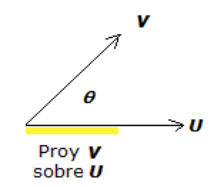
\includegraphics[width=0.30\textwidth]{imagenes/imagenes10/T10IM07.png}
\end{figure}
\end{multicols}


	Propiedad fundamental: $\forall \  \vec u,\ \vec v\ \neq 0:\ \boxed{\  \vec u \bot \vec v \ \leftrightarrow \ \vec u \cdot \vec v=0 \ }$
		
	$\vec u \cdot \vec v = \vec v \cdot \vec u$; $\ \alpha ( \vec u \cdot \vec v) =( \alpha \vec u) \cdot \vec v = \vec u \cdot ( \alpha \vec v)$; $\ \vec u \cdot (\vec v + \vec w)= \vec u \cdot \vec v + \vec u \cdot \vec w$
		
	 Módulo de un vector: $\boxed{ \ | \vec u |=+\sqrt{\vec u \cdot \vec u} \ }$
		
	 Ángulo entre dos vectores: $\boxed{ \ \cos \theta = \dfrac {\vec u \cdot \vec v}{|\vec u| \cdot |\vec v|} \ }$
	 
\vspace{4mm} \textbf{Producto escalar en B.O.N. \small{(Base orto-normal)}}

$BON=\{ \vec i, \vec j, \vec k \ / \  |\vec i|=|\vec j|=|\vec k|=1 \ \wedge \ \vec i \bot \vec j; \ \vec j \bot \vec k; \ \vec k \bot \vec i \}$. 

$\vec u=(u_1,u_2,u_3); \ \vec v=(v_1, v_2, v_3) \ \to \ $
$\boxed{  \ \vec u \cdot \vec v= u_1 v_1+u_2 v_2+u_3 v_3 \ }  \  \in \mathbb{R}$

\vspace{2mm} Módulo en una BON: $ \vec u=(u_1,u_2,u_3) \to |\vec u|=+\sqrt{u_1^2+u_2^2+u_3^2}$
		
\vspace{2mm} Ángulo \small{de dos vectores en una BON:} $\cos \theta = \dfrac {u_1 v_1+u_2 v_2+u_3 v_3}{\sqrt{u_1^2+u_2^2+u_3^2}\cdot \sqrt{v_1^2+v_2^2+v_3^2}}$

\vspace{4mm}

\begin{multicols}{2}
\textit{Normalización de un vector:} 

Dado un vector $\vec v$, conseguir otro de la misma dirección pero de módulo $1$, le llamaremos $\vec u_v$ y se obtiene como: $\vec u_v=\dfrac {1}{|\vec v|}\cdot \vec v = (\cos \alpha, \cos \beta, \cos \gamma)$, son los llamados \textit{cosenos directores} (las componentes de todo vector unitario).
\begin{figure}[H]
	\centering
	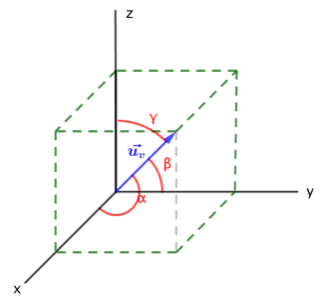
\includegraphics[width=0.30\textwidth]{imagenes/imagenes10/T10IM08.png}
\end{figure}
\end{multicols}

\subsection{Producto `Vectorial'}

El producto vectorial de dos vectores $\vec u$ y $\vec v$ es un nuevo vector $\vec u \times \vec v$	 tal que:
\begin{multicols}{2}
\begin{itemize}
\item su módulo es $|\vec u \times \vec v|=|\vec u||\vec v| \sin \theta $, siendo $\theta$ el ángulo que forman $\vec u$ y $\vec v$.
\item su dirección es perpendicular al plano que forman $\vec u$ y $\vec v$.
\item y su sentido es el del giro de un `sacacorchos' que intente llevar el vector$\vec u$ hacia el $\vec v$.
\end{itemize}
\begin{figure}[H]
	\centering
	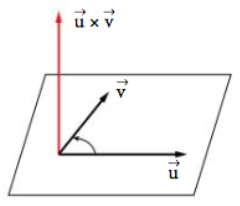
\includegraphics[width=0.30\textwidth]{imagenes/imagenes10/T10IM09.png}
\end{figure}
\end{multicols}

\textbf{Propiedades del producto vectorial.}
\begin{multicols}{2}

El \underline{módulo} del producto vectorial mide el \underline{área del paralelogramo} que forman los vectores $\vec u$ y $\vec v$.
				
\hspace{10mm}$|\vec u \times \vec v|=|\vec u||\vec v| \sin \theta$

\begin{figure}[H]
	\centering
	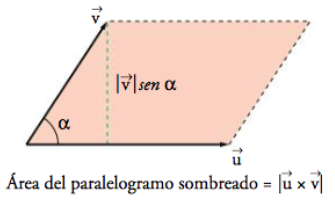
\includegraphics[width=0.30\textwidth]{imagenes/imagenes10/T10IM10.png}
\end{figure}

\end{multicols}

\begin{itemize}
	\item ¡El producto vectorial es \underline{no-conmutativo}!: $\vec u \times \vec v=-\vec v \times \vec u$
	\item $\vec u \times \vec u=\vec 0$
	\item Tomaremos la BON \underline{orientada}, $\vec i \times \vec j = \vec k$; $\vec j \times \vec k = \vec i$ y $\vec k \times \vec i = \vec j$

A esto es lo que llaman los físicos una BON `orientada', los vectores $\vec i, \vec j, \vec k$ no pueden tener orientaciones cualesquiera. 	

\item $(\alpha \vec u)\times \vec v=\alpha (\vec u \times \vec v)= \vec u \times (\alpha \vec v)$
\item ¡\underline{No} se cumple la \underline{asociativa}!: $\vec u \times (\vec v \times \vec w) \neq (\vec u \times \vec v)\times \vec w$
\item \underline{Distributivas}: $\vec u \times (\vec v + \vec w)= \vec u \times \vec v + \vec u \times \vec w$; $(\vec u + \vec v)\times \vec w=\vec u \times \vec w + \vec v \times \vec w$
\item En componentes, el desarrollo del producto vectorial es un determinante:
\begin{equation}		
\boxed{ \ \overrightarrow { u } \times \overrightarrow { v } \quad =\quad \left| \begin{matrix} \overrightarrow { i }  & \overrightarrow { j }  & \overrightarrow { k }  \\ u_1 & u_2 & u_3 \\ v_1 & v_2 & v_3 \end{matrix} \right| \ }
\end{equation}
\end{itemize}
		
\vspace{2mm}$\vec u \times \vec v$ siempre es un vector perpendicular a $\vec u$ y a $\vec v$ y su módulo representa el área del paralelogramos que defines estos dos vectores.

\vspace{5mm} ¡ Afortunadamente, el producto vectorial no es asociativo XD !

\begin{figure}[H]
	\centering
	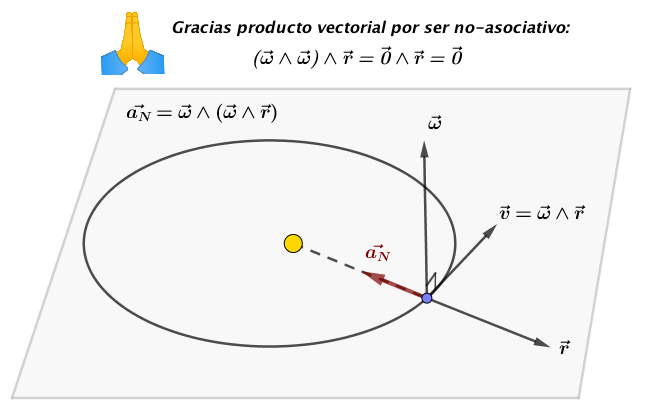
\includegraphics[width=1\textwidth]{imagenes/imagenes10/T10IM11.png}
\end{figure}

\subsection{Producto `Mixto'}
\begin{equation}
\boxed{ \ [\vec u, \vec v, \vec w]=\vec u \cdot (\vec v \times \vec w)=|\vec u|\cdot|(\vec v \times \vec w)|\cdot \cos \theta \ }
\end{equation}

\begin{multicols}{2}
El \underline{producto mixto} $[\vec u, \vec v, \vec w]$ mide, \underline{en valor absoluto}, el \underline{volumen del paralelepípedo} formado por los tres vectores.
				
En componentes se calcula como un determinante:
				
$\boxed{ \ [\overrightarrow { u } ,\overrightarrow { v }, \overrightarrow { w }]  \quad =\quad \left| \begin{matrix} u_{ 1 } & u_{ 2 } & u_{ 3 } \\ v_{ 1 } & v_{ 2 } & v_{ 3 } \\ w_{ 1 } & w_{ 2 } & w_{ 3 } \end{matrix} \right| \ } $

\begin{figure}[H]
	\centering
	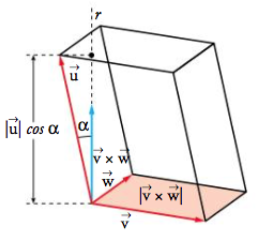
\includegraphics[width=0.40\textwidth]{imagenes/imagenes10/T10IM12.png}
\end{figure}
\end{multicols}

\begin{multicols}{2}
Por propiedades de los determinantes y del valor absoluto podemos afirmar que para el cálculo del volumen de un paralelepípedo formado por tres vectores no importa el orden en que los cojamos para calcular el producto mixto.
\begin{figure}[H]
	\centering
	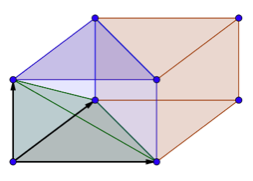
\includegraphics[width=0.20\textwidth]{imagenes/imagenes10/T10IM13.png}
\end{figure}
\end{multicols}


\subsection{Ejercicios resueltos de repaso de geometría vectorial}


\begin{ejer}
	Obtén 3 vectores perpendiculares a $\vec u=(3,2,7)$, no proporcionales entre sí
\end{ejer}

\begin{proofw}\renewcommand{\qedsymbol}{$\diamond$}.
	
	\begin{multicols}{2}
	Sabemos que  
	$  \vec u \bot \vec v \ \leftrightarrow \ \vec u \cdot \vec v=0 \ $
	y que vectores perpendiculares a uno dado hay infinitos (todo un `plano vectorial'), y que cualquier combinación de dos vectores perpendiculares a uno dado también es perpendicular a éste.
	\begin{figure}[H]
	\centering
	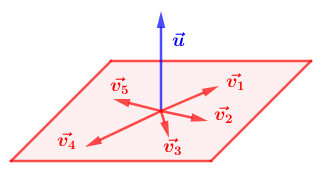
\includegraphics[width=0.30\textwidth]{imagenes/imagenes10/T10IM15.png}
	\end{figure}	
	\end{multicols}	
	Solo tenemos que encontrar vectores $\vec {v_i}$ tales que $\vec u \cdot \vec {v_i}=0$. Por ejemplo:
	
	$\vec {v_1} = (0,-7,2) \to \vec u \cdot \vec {v_1}=(3,2,7)\cdot (0,-7,2)=3 \cdot 0 + 2 \cdot (-7) + 7 \cdot 2 =-14+14=0$
	
	Compruébese que $\ \vec {v_2} = (7,0,-3);  \quad \vec {v_3} = (2,-3,0) \ $ también son perpendiculares a $\vec u$
	
	También es perpendicular a $\vec u$ cualquier combinación lineal de estos tres vectores encontrados, como p.e.:
	$\ \vec {v_4}  = \vec {v_2}+\vec {v_3}= (9,-3-3)$; incluso si lo simplificamos dividiendo por 3 (multiplicar un vector por $\frac 1 3 $  proporciona un vector de la misma dirección: $\vec {v'_4}=(3,-1,-1) \to   \ \vec u \bot \vec {v'_4} $ (\emph{compruébese}).
	
	Otro más: $\vec {v_5}=\vec {v_1} - 2 \vec {v_2}+ 3\vec {v_3}= (8,-18,8)$ (\emph{compruébese}).
\end{proofw}


\begin{ejer}

	Dados:  $\vec u=(1,0,-1); \vec v=(2,3,1)$. Calcular $u \cdot v; |u|; |v|; \cos \theta $
\end{ejer}


\begin{proofw}\renewcommand{\qedsymbol}{$\diamond$}
.

$u \cdot v = (1,0,-1) \cdot (2,3,1)=2+0-1=1$

$|\vec u|=+\sqrt{1^1+0^2+(-1)^2}=\sqrt{2}\; ; \quad |\vec v|=+\sqrt{2^2+3^2+1^2}=\sqrt{14}$

$\vec u \cdot \vec v = |\vec u|\cdot |\vec v| \cdot \cos \theta \to 
1=\sqrt 2 \, \sqrt{14} \; \cos \theta \to \cos \theta = \frac {\sqrt{7}}{14} \textcolor{gris}{\to \theta=79.1^o}  $

	
\end{proofw}


\begin{ejer}
	Obtén un vector perpendicular a $\vec u=(3,-1,2)$ y  a $\vec v=(1,0,3)$.
\end{ejer}

\begin{proofw}\renewcommand{\qedsymbol}{$\diamond$}
	
	Lo más sencillo es buscar el vector producto vectorial de ambos: $ \vec w =\vec u \times \vec v$
	
	$\overrightarrow { w } =\left| \begin{matrix} \vec { i }  & \vec { j }  & \vec { k }  \\ 3 & -1 & 2 \\ 1 & 0 & 3 \end{matrix} \right| =[\text{ Sarrus }] =-3\vec { i } -7\vec { j } +\vec { k } =(-3,-7,1)$
\end{proofw}


\begin{ejer}
	Calcula el área del rectángulo de vértice  $A(2,3,7), B(1,-5,4)\  y\  C(7,0,11)$
\end{ejer}

\begin{proofw}\renewcommand{\qedsymbol}{$\diamond$}
	
	Con los vértices $A, B,$ y $C$, formamos los vectores $\vec u=\overrightarrow {AB}$ y $\vec v=\overrightarrow {AC}$. Por definición del producto vectorial, el área del triángulo será igual a $ \frac 1 2 \; | \vec u \times \vec v |$

$\vec u=\overrightarrow {AB}=B-A=(-1,-8,-3)$ y $\vec v=\overrightarrow {AC}= C-A=(5, -3, 4)$.

$\overrightarrow { u \times v } =\left| \begin{matrix} \vec { i }  & \vec { j }  & \vec { k }  \\ -1 & -8 & -3 \\ 5 & -3 & 4 \end{matrix} \right| ==-41\vec { i } -11\vec { j } +43\vec { k } =(-41,-11,43)$

$|\overrightarrow { u \times v } | = \sqrt{(-41)^2+(-11)^2+(43)^2}\approx 60.42$

Área triángulo $ \approx  \frac 1 2 \; 60.41 = 30.21\; u^2$

¡Atención!: si al calcular el área de un triángulo dado por sus tres vértices el resultado es cero $\to$ ' los tres puntos están alineados'.
\end{proofw}

%5
\begin{ejer}
	Calcula el volumen del tetraedro cuyos vértices son: $A(-7,-2,5), B(0,2,0), C(-9,3,8)$  y $D(-7,5,9)$; 
\end{ejer}

\begin{proofw}\renewcommand{\qedsymbol}{$\diamond$}

Formamos los vectores:

$\vec u = \overrightarrow {AB}=B-A=(7,4,-5)$; 
$\vec v = \overrightarrow {AC}=C-A=(-2,5,3)$; 
$\vec w = \overrightarrow {AD}=D-A=(0,7,4)$

Sabemos que el valor absoluto del producto mixto de estos tres vectores es el volumen del paralelepípedo que forman, que su mitad es el volumen del prima y la sexta parte la del tetraedro, que es lo que nos piden, así que: 

Volumen tetraedro = $\frac 1 6 \left|\;  \left[ vec\quad u,\quad vec\quad v,\quad vec\quad w \; \right] \right|  =\left| \;  \left| \begin{matrix} 7 & 0 & 3 \\ -2 & 5 & 3 \\ 0 & 7 & 4 \end{matrix} \right|\;  \right| =\frac 1 6 \; |95|= \frac {95}{6} \; u^2$	
\end{proofw}


\begin{ejer}
	Calcula el volumen de paralelepípedo (y del prisma y del tetraedro) formado por los vectores libres $\vec u=(3,1,2), \vec v=(4,-1,0)\  y\  \vec w=(3,6,2)$
\end{ejer}

\begin{proofw}\renewcommand{\qedsymbol}{$\diamond$}
	
	$\left[ vec\quad u,\quad vec\quad v,\quad vec\quad w \right] =\left| \begin{matrix} 3 & 1 & 2 \\ 4 & -1 & 0 \\ 3 & 6 & 2 \end{matrix} \right| =40$
	
	$Vol_{paral}  = 40 \;  u^3; \quad  Vol_{prism} = \frac {40}2 =20\; u^3; \quad Vol_{tetr} = \frac {40}6 = 20/3 \; u^3$
	
\end{proofw}


\begin{ejer}
	Calcular él ángulo que forman dos diagonales de un cubo.
\end{ejer}

\begin{proofw}\renewcommand{\qedsymbol}{$\diamond$}
\begin{multicols}{2}	
	\begin{figure}[H]
	\centering
	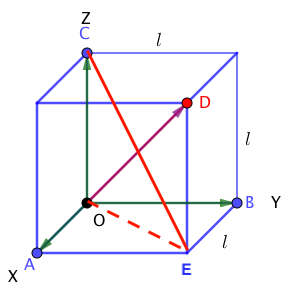
\includegraphics[width=0.30\textwidth]{imagenes/imagenes10/T10IM16.png}
	\end{figure}
De las 4 diagonales del cubo (no diagonales de las caras), elegimos las de la figura, con vectores asociados: $\overrightarrow{OD}=D-O=(l,l,l)-)0,0,0)=(1,1,1)\; l\; $ y $\overrightarrow{EC}=C-E=(0,0,l)-(l,l,0)=(1,-1,-1)\; l$

Calcule el lector el ángulo entre estos vectores con ayuda del producto escalar. \scriptsize{( $\theta \approx 109.5^0$, las diagonales, como rectas: $180-109.5=	70.5^0$)}

\end{multicols}
\end{proofw}



\section{Introducción al cálculo vectorial}

Para el desarrollo de esta sección me he basado en los apuntes anónimos encontrados en `http://www.cartagena99.com/recursos/examenes-ejercicios-apuntes.php' : ``Apuntes de: campos escalares y vectoriales''. También he usado los apuntes de Beléndez, Bernabeu y Partor, `Magnitudes, vectores y campos' de la UPV y encontrado en la web. Mi gratitud a todos los que comparten material en la red.

\subsection{Vector función de un escalar}

\begin{multicols}{2}
Un vector $\vec r$ es función de un escalar (número real) $t$ si lo es alguna de sus componentes:

$\boxed{ \; \vec r(t)=r_x(t) \vec i + r_y(t) \vec j + r_z(t) \vec k \; } \quad$
Tenemos una función de $\mathbb R \to \mathbb R^3\; : \; t \leadsto \vec {r(t)}$. 

Si tomamos todos los vectores con origen en $O$, sus extremos, para los distintos valores de $t$, dibujan una curva llamada `indicatriz' de ecuaciones paramétricas: $r_x=r_x(t); \; r_y=r_y(t); \; r_z=r_z(t)$. Si $t$ es el tiempo y $\vec r$ el vector de posición de una partícula, la `indicatriz' $ \vec r (t)$ será la `trayectoria'.

	\begin{figure}[H]
	\centering
	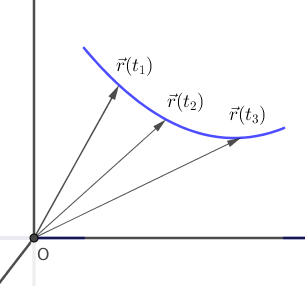
\includegraphics[width=0.4\textwidth]{imagenes/imagenes10/T10IM17.png}
	\end{figure}
\end{multicols}

\subsection{Derivada e integral de un vector}

\begin{multicols}{2}
	\begin{figure}[H]
	\centering
	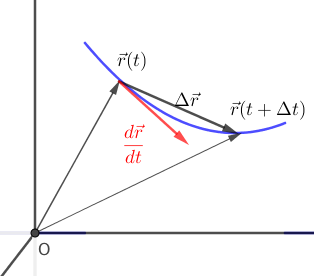
\includegraphics[width=0.4\textwidth]{imagenes/imagenes10/T10IM18.png}
	\end{figure}
Al pasar de $t$ a $t+ \Delta t \to \vec r (t)$ para a $\vec r (t+\Delta t)$ Si se incrementa la variable $t$ se incrementará el vector $\vec r$:

$\vec r (t) + \Delta \vec r = \vec r (t+\Delta t) = r_x (t+\Delta t) \vec i + r_y (t+\Delta t) \vec j + r_z (t+\Delta t) \vec k$

Despejando: $\Delta r =\vec r (t+\Delta t) - \vec r (t) = \Delta r_x \vec i +\Delta r_y \vec j +\Delta r_z \vec k \; $;  donde $\Delta r_x =  r_x (t+\Delta t) -  r_x (t) $ y análogamente para $\Delta r_y$ y $\Delta r_z$.
\end{multicols}

$\dfrac {\dd \vec r}{\dd t }= \underset{\Delta t \to 0}{lim}\; {\dfrac {\Delta r_x}{\Delta t}\;  \vec i} + \underset{\Delta t \to 0}{lim}\; {\dfrac {\Delta r_y}{\Delta t}\;  \vec j} + \underset{\Delta t \to 0}{lim}\; {\dfrac {\Delta r_z}{\Delta t}\;  \vec k}$

Es decir, la derivada de un vector respecto de un escalar es un vector cuyas componentes son las derivadas respecto del escalar de las respectivas componentes del vector a derivar.

\hspace{30mm}$\boxed{ \; \dfrac {\dd \vec r}{\dd t }= \overrightarrow {r'} = \dfrac {\dd r_x}{\dd t}\; \vec i + \dfrac {\dd r_y}{\dd t}\; \vec j + \dfrac {\dd r_z}{\dd t}\; \vec k\; }$

Por la interpretación geométrica de la derivada (\ref{IG-derivada}),el vector derivada es tangente a la curva indicatriz (trayectoria) (la dirección secante $\Delta \vec r$, con $\Delta t \to 0$ tiende a la dirección de la tangente $  \overrightarrow { r'} =\dfrac {\dd \vec r}{\dd t }\;$).

\vspace{4mm} \textbf {Reglas de derivación.} 

\begin{enumerate}[a) ]
\item Derivada de la suma de vectores: 
$\quad \dfrac {\dd {(\vec r + \vec s)}}{\dd t }$
$=\dfrac {\dd \vec r}{\dd t }+\dfrac {\dd \vec s}{\dd t }$

\item Derivada del producto por un escalar: $\quad \dfrac {\dd {(k\cdot \vec r)}}{\dd t }= k\cdot \dfrac {\dd \vec r}{\dd t }$
\item Derivada del producto escalar de dos vectores: $\quad \dfrac {\dd (\vec r \cdot \vec s)}{\dd t } = \dfrac {\dd \vec r}{\dd t }\cdot \vec s + \vec r \cdot \dfrac {\dd \vec s}{\dd t }$
\item Derivada del producto vectorial: $\dfrac {\dd (\vec r \times \vec s)}{\dd t }= \dfrac {\dd \vec r}{\dd t }\times \vec s + \vec r \times \dfrac {\dd \vec s}{\dd t }$	
\end{enumerate}

\underline{Propiedad} si $\vec r$ tiene módulo constante $\to$ es perpendicular a su vector derivada.

\begin{proofw}\renewcommand{\qedsymbol}{$\diamond$}

Si $\vec r (t)$ tiene módulo cte. $\vec r (t) \cdot \vec r (t)= r^2 =cte.$. Derivado este producto escalar:

$\quad \dfrac {\dd (\vec r \cdot \vec r)}{\dd t }=2\vec r \cdot \dfrac {\dd \vec r}{\dd t}=0$, ya que $\dfrac {\dd \; cte}{\dd t}=0 \Rightarrow \; \boxed{\; |\vec r|=cte \leftrightarrow \displaystyle \vec r \; \bot \;  \dfrac {\dd \vec r}{\dd t }\;} $
\end{proofw}

\vspace{4mm} \textbf{Integral de un vector}. Se define como la operación inversa a la derivada de un vector: la integral de un vector $\vec r(t)=r_x(t) \vec i + r_y(t) \vec j + r_z(t) \vec k$ es otro vector cuyas componentes son las integrales de las componentes del primero.

\hspace{20mm} $\boxed{ \; \displaystyle \int \vec r (t)\; \dd t = \vec i \; \int r_x (t)\; dd t + \vec j \; \int r_y (t)\; dd t+ \vec k \; \int r_z (t)\; dd t \; }$

\subsection{Campos escalares}

Una función escalar $\phi$ que toma valores en los puntos $x,y,z)$ del espacio se dice que es una función escalar de punto o, más simplemente, un `campo escalar' si:

A cada punto $P(x,y,z)$ del espacio, la función $\phi$ le asocia un número $\phi (x,y,z)\in \mathbb R$, es una aplicación de $\mathbb R^3$ en $\mathbb R$.

Ejemplos físicos de campos escalares son la temperatura (T), la presión (P), el potencial eléctrico (V), etc. 

El conjunto de todos los puntos del plano donde el campo $\phi$ toma un determinado valor $\phi_0$ forman una `superficie equiescalar', de ecuación: $\phi=\phi_0$.

\begin{multicols}{2}
Las superficies equiescalares pueden representar puntos que están a la misma temperatura (isotermas), a la misma presión (isóbaras), al mismo potencial eléctrico (superficies equipotenciales), etc.

\footnotesize{Si el campo esta definido en un plano las equiescalares serán líneas en vez de superficies. Como ejemplo, piénsese en las curvas de nivel de un mapa topográfico, $H(x,y)$ es la altura del punto $P(x,y)$ del mapa-2D}.

	\begin{figure}[H]
	\centering
	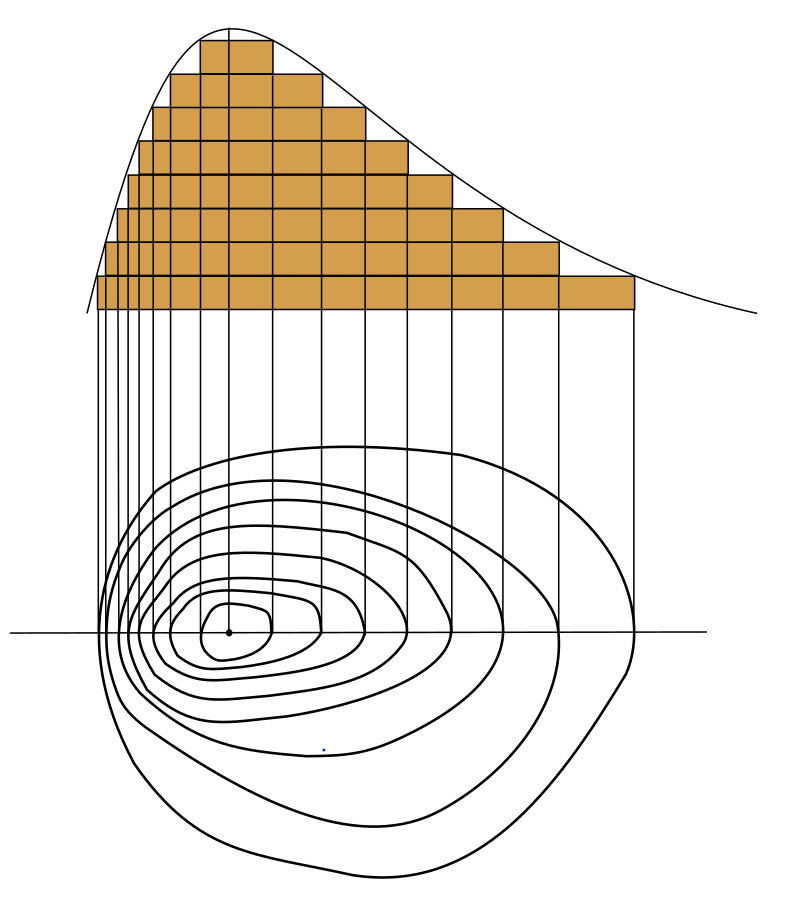
\includegraphics[width=0.3\textwidth]{imagenes/imagenes10/T10IM19.png}
	\end{figure}
\end{multicols}
\normalsize
En las funciones de una sola variable $y=f(x)$, la derivada (Leibniz) se define como el límite al que tiende el cociente $\Delta y / \Delta x$ cuando $\Delta x \to 0$, pero  un campo escalar $\phi (x,y,z)$ tendrá distintas derivadas ya que puede incrementarse una variable u otra, así, se define el crecimiento a lo largo del eje $OX$ como: $\Delta \phi_x =\phi (x+\Delta x, y, z)- \phi(x,y,z)$. Y su derivada, respecto de esta variable x, que se denota por $\dfrac{\partial \phi}{\partial x} = \underset {\Delta x \to 0}{lim}\;{\dfrac {\Delta \phi_x}{\Delta x}}= \eval {\dfrac {\dd \phi}{\dd x}}_{y,z=ctes.}\; \; $. Es decir, se trata de la derivada que resulta de suponer que $y$ y $z$ permanecen constantes y solo varía $x$. Análogamente se definen: $\dfrac{\partial \phi}{\partial y}=\eval {\dfrac {\dd \phi}{\dd y}}_{x,z=ctes.}\; $ y $\; \; \dfrac{\partial \phi}{\partial z}=\eval {\dfrac {\dd \phi}{\dd z}}_{x,y=ctes.}\; $. Esto es lo que se llama \underline{`derivadas parciales'}.

Las reglas de la derivación parcial son las mismas que para las funciones de una variable, solo hay que considerar que la variable sobre la que se deriva es realmente una variable y considerar al resto de vbles. como ctes.

Derivadas parciales: $\quad \boxed{\; \dfrac{\partial \phi}{\partial x}=\eval {\dfrac {\dd \phi}{\dd x}}_{y,z=ctes.} \quad \dfrac{\partial \phi}{\partial y}=\eval {\dfrac {\dd \phi}{\dd y}}_{z,x=ctes.} \quad \dfrac{\partial \phi}{\partial z}=\eval {\dfrac {\dd \phi}{\dd z}}_{x,y=ctes.} \;} $

\section{Campos Vectoriales}
\begin{multicols}{2}
	En matemáticas, un campo vectorial representa la distribución espacial de una magnitud vectorial. Es una expresión de cálculo vectorial que asocia un vector a cada punto en $\mathbb R^3$, de la forma $\vec E: \mathbb R^3 \to \mathbb R^3 \; : \vec E (x,y,z)= E_x \vec i + E_y \vec j + E_z \vec k$
	
	Los campos vectoriales se utilizan en física, por ejemplo, para representar la velocidad y la dirección de un fluido en el espacio, o la intensidad y la dirección de fuerzas como la gravitatoria o la fuerza electromagnética.
	
	\begin{figure}[H]
	\centering
	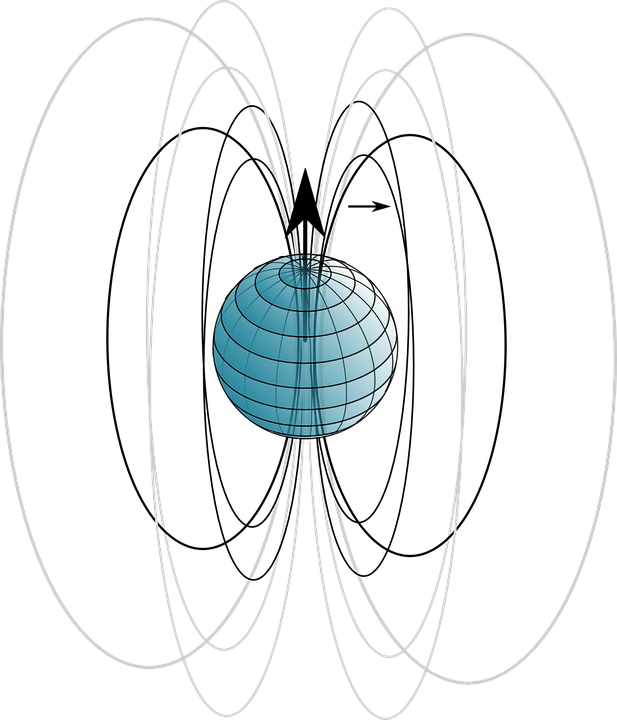
\includegraphics[width=0.4\textwidth]{imagenes/imagenes10/T10IM20.png}
	\end{figure}
\end{multicols}

\section{Gradiente de un campo escalar}

Sea $\phi (x,y,z)$ una función escalar, definida y derivable en cada uno de los puntos $(x.y.z)$ de una cierta región del espacio ($\phi$ es un campo escalar derivable), el `gradiente' de $\phi$, representado por $\overrightarrow {grad}\;  \phi\; $ o   $\; \overrightarrow{\nabla} \phi$ es un vector que se obtiene por la fórmula:

\vspace{4mm}\centerline{ $\boxed{ \; \overrightarrow {grad} \; \phi =  \overrightarrow {\nabla} \phi = \dfrac {\partial \phi}{\partial x}\; \vec i +  \dfrac {\partial \phi}{\partial y}\; \vec j +  \dfrac {\partial \phi}{\partial z}\; \vec k   \;} $}

Nótese que $\overrightarrow {grad} \; \phi $ define un `campo vectorial', es un vector que indica como varía $\phi$ en las proximidades de un punto, con el sentido del máximo crecimiento de la función.

Matemáticamente, la diferencial de una función $\phi (x.y.z)$ viene dada por:

\vspace{4mm}\centerline {$\boxed{ \; \dd \; \phi = \dfrac {\partial \phi}{\partial x}\; \dd x +  \dfrac {\partial \phi}{\partial y}\; \dd y + \dfrac {\partial \phi}{\partial z}\; \dd z \; }$}

\vspace{2mm} En notación de Leibniz, $\dd \phi$ representa la variación de $\phi$ entre dos puntos muy próximos: $x,y,z)\; $ y $\; (x+\dd x. y +\dd y, z +\dd z)$. Teniendo en cuenta la definición de gradiente:

$\dd \; \phi = \dfrac {\partial \phi}{\partial x}\; \dd x +  \dfrac {\partial \phi}{\partial y}\; \dd y + \dfrac {\partial \phi}{\partial z}\; \dd z = \left( \dfrac {\partial \phi}{\partial x}\; \vec i + \dfrac {\partial \phi}{\partial y}\; \vec j + \dfrac {\partial \phi}{\partial z}\; \vec k     \right) \cdot (\dd x \; \vec i + \dd y \; \vec j + \dd z \; \vec k)$
\begin{multicols}{2}
\vspace{3mm} Es decir: $\quad \boxed {\; \dd\; \phi = \overrightarrow {grad}\; \phi \cdot \dd \; \vec r = \overrightarrow { \nabla} \; \phi \cdot \dd \; \vec r \;} \quad$, donde $\dd \; \vec r = \dd x \; \vec i +\dd y \; \vec j + \dd z \; \vec k$, vector que une los puntos anteriormente señalados (desplazamiento infinitesimal). Esta ecuación determina la variación  $\dd \; \phi$ de la función escalar $\phi$ a lo largo de la dirección $\dd \; \vec r$. Des esta ecuación se deduce:

$\dd \; \phi = |\overrightarrow{\nabla}\; \phi |\cdot |\dd \vec r|\cdot \cos \theta$

	\begin{figure}[H]
	\centering
	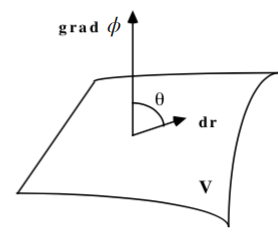
\includegraphics[width=0.4\textwidth]{imagenes/imagenes10/T10IM21.png}
	\end{figure}
\end{multicols}
deducimos que, para que exista una máxima variación del campo, para un valor fijo $|\dd \vec r|$, ha de ocurrir que 
$\cos \theta=1 \to \theta = 0\; $:  

\vspace{3mm}
\fbox{ \parbox{0.9\linewidth}{\emph{`El gradiente tiene la dirección de la máxima variación del campo y va en el sentido creciente de $\phi$'}}}
\vspace{3mm}

Las componentes del gradiente $\overrightarrow {\nabla} \; \phi$ en la dirección de un vector unitario $\overrightarrow {u_N}$ es igual al producto escalar $\overrightarrow {\nabla} \; \phi \cdot \overrightarrow {u_N} $ y se llama \textbf{derivada direccional} de $\phi$ en la dirección de $\overrightarrow {u_N}$ :

\centerline {$\boxed{\; \dfrac {\partial \phi}{\partial \overrightarrow {u_N}} = \overrightarrow {u_N} \cdot \overrightarrow {\nabla \phi}  \; }$}

\begin{multicols}{2}
Para una superficie $S$ determinada por la ecuación $f(x,y,z)=0$, el vector unitario normal en el punto $(x,y,z)$ viene dado por:

\hspace{15mm} $\overrightarrow {u_N}= \dfrac {\overrightarrow {\nabla f}}{|\overrightarrow {\nabla f}|}$

	\begin{figure}[H]
	\centering
	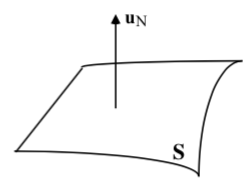
\includegraphics[width=0.35\textwidth]{imagenes/imagenes10/T10IM22.png}
	\end{figure}
\end{multicols}

La expresión: $ \overrightarrow {\nabla} \phi = \dfrac {\partial \phi}{\partial x}\; \vec i +  \dfrac {\partial \phi}{\partial y}\; \vec j +  \dfrac {\partial \phi}{\partial z}\; \vec k\;$, se puede obtener como el producto de un `operado vectorial' por un escalar , es decir:
$ \overrightarrow {\nabla} \phi = \left( \dfrac {\partial }{\partial x}\; \vec i +  \dfrac {\partial }{\partial y}\; \vec j +  \dfrac {\partial }{\partial z}\; \vec k \right) \cdot \phi\;$.
 El término dentro del paréntesis recibe el nombre de \textbf{`operado nabla'}:

\vspace{4mm}

\centerline{ $\boxed{ \; \overrightarrow {\nabla}=  \dfrac {\partial }{\partial x}\; \vec i +  \dfrac {\partial }{\partial y}\; \vec j +  \dfrac {\partial }{\partial z}\; \vec k \; }$}

\vspace{3mm}En resumen, el gradiente de una función escalar es un campo vectorial que tiene las siguientes propiedades:

 \begin{enumerate}

\item Sus componentes, en cada punto, son la razón de las variaciones de la función y de la coordenada a lo largo de las direcciones de los ejes en dicho punto. 

\item Su módulo, en cada punto, es el máximo valor de la variación de la función con la distancia. 

\item Su dirección es la de máxima variación. 

\item Su sentido es el de crecimiento de la función.

 \end{enumerate}
 
 El gradiente es, por tanto, un campo vectorial de punto deducido de un campo escalar de punto.
 
 \subsection{Divergencia de un campo vectorial}
 
 Sea $\vec E (x,y,z)=E_x \vec i + E_y \vec j + E_z \vec k\;$, una función vectorial definida y derivable en los puntos de una determinada región del espacio, $\vec E$ es un campo vectorial derivable.
 
 La divergencia de $\vec E$, representada por $div\; \vec E\;$ ó $\overrightarrow{\nabla}\cdot \vec E$, viene dada por la expresión:
 
 \vspace{4mm}\centerline{$\boxed{\; div\; \vec E = \overrightarrow{\nabla}\cdot \vec E = \dfrac {\partial E_x}{\partial x } + \dfrac {\partial E_y}{\partial y }+ \dfrac {\partial E_z}{\partial z } \; }$} 
 
 \vspace{3mm} que puede interpretarse como el `producto escalar' del operador $\overrightarrow{\nabla}$ por el campo vectorial $\vec E$, en ese orden y es, evidentemente, un escalar.
 
	La divergencia nos permite caracterizar aquellos puntos del campo vectorial en que éste, valga la expresión, `se crea o se destruye'; es decir, clasifica los manantiales o sumideros del campo. 

	Cuando $div \; \vec E = 0$ , no hay fuentes escalares del campo $\vec E$ , y se dice que el campo vectorial $\vec E$ es \textbf{\emph{solenoidal}}. 

	Si no existen `fuentes escalares' del campo éste no podrá `nacer` o `morir' en dichas fuentes, por lo cual las líneas del campo solenoidal son siempre cerradas. 

\subsection{Rotacional de un campo vectorial}

Sea $\vec E (x,y,z)=E_x \vec i + E_y \vec j + E_z \vec k\;$, un campo vectorial derivable, el rotacional de $\vec E$ , representado por $rot \; \vec E\; $ ó $\overrightarrow{\nabla} \times \vec E$ viene dado por la expresión:

\vspace{4mm} $rot \; \vec E = \overrightarrow{\nabla} \times \overrightarrow {E} = \left| \begin{matrix} \vec { i }  & \vec { j }  & \vec { k }  \\ \frac { \partial  }{ \partial x }  & \frac { \partial  }{ \partial y }  & \frac { \partial  }{ \partial z }  \\ \quad E_{ x } & E_{ y } & E_{ z } \end{matrix} \right| $
$=\tiny{\left( \dfrac{\partial E_z}{\partial y} -\dfrac{\partial E_y}{\partial z} \right) \; \vec i + \left(\dfrac{\partial E_x}{\partial z} -\dfrac{\partial E_z}{\partial x} \right)\; \vec j+ \left(\dfrac{\partial E_y}{\partial x} -\dfrac{\partial E_x}{\partial y} \right)\; \vec k}$

\vspace{3mm}El rotacional de un vector puede entenderse como el `producto vectorial' del operador $\overrightarrow{\nabla}$ por el campo vectorial $\overrightarrow{E}$, en ese orden.

Cuando $\overrightarrow{\nabla} \times \overrightarrow {E}=\overrightarrow{0}$, se dice que el campo es \textbf{`ìrrotacional'} y nos permite decir que en campo $\overrightarrow {E}$ proviene de una función escalar $\phi$, en la forma:

$\overrightarrow{\nabla} \times \overrightarrow {E}=\overrightarrow{0} \longrightarrow \overrightarrow{E}-\overrightarrow{\nabla}\; \phi=-\overrightarrow{grad}\; \phi$

El valor del rotacional de un campo vectorial nos da las `fuentes vectoriales' del campo en cada punto. Si $\overrightarrow{\nabla} \times \overrightarrow {E}=\overrightarrow{0}$ para todos los puntos, entonces $\overrightarrow{E}$ no tiene fuentes vectoriales.

\subsection{Laplaciana de una función escalar}

Sea $\phi \; (x,y,z)$ un campo escalar definido u dos veces derivable en una determinada región del espacio. La laplaciana de $\phi$, representada por $\triangle\; \phi \;$ ó $\; \nabla^2 \; \phi$, lo determina la expresión:

\vspace{4mm}\centerline{$\boxed{\;\triangle\; \phi= \nabla^2 \; \phi =  \dfrac{\partial^2\; \phi}{\partial x^2}+\dfrac{\partial^2\; \phi}{\partial y^2}+\dfrac{\partial^2\; \phi}{\partial z^2} \;}$}

\vspace{3mm} La laplaciana es una función escalar.

Análogamente al `operador nabla', podemos definir el \textbf{`operador laplaciana'} como:


\vspace{4mm}\centerline{$\boxed {\;	\triangle = \nabla^2 = \dfrac {\partial^2}{\partial x^2}+ \dfrac {\partial^2}{\partial y^2}+\dfrac {\partial^2}{\partial z^2} \; }$}

Cuando el campo escalar $\phi$ tiene derivadas segundas continuas y se cumple $\triangle \; \phi = 0$, entonces se dice que el campo escalar $\phi$ es un `campo armónico'. La ecuación  $\triangle \; \phi = 0$ se llama \textbf{ecuación de Laplace}.

% *********************. Revisado el tema hasta aquí. 

\section{Ejercicios}

\begin{ejre}
Dado el campo vectorial $\overrightarrow A =x^2 \; \vec i + \sin y \; \vec j + zx \; \vec k$, encuentra: $\overrightarrow {\nabla} \cdot \overrightarrow A; \quad \overrightarrow \nabla \; (\overrightarrow {\nabla} \cdot \overrightarrow A); \quad \overrightarrow {\nabla} \times \overrightarrow A$	
\end{ejre}

\vspace{3mm}\begin{proofw}\renewcommand{\qedsymbol}{$\diamond$}.	 

$\overrightarrow{\nabla}\cdot \vec A = \dfrac {\partial A_x}{\partial x } + \dfrac {\partial A_y}{\partial y }+ \dfrac {\partial A_z}{\partial z } = 3x+\cos y$	

$\overrightarrow \nabla \; (\overrightarrow {\nabla} \cdot \overrightarrow A)= \overrightarrow \nabla (3x+\cos y)= \dfrac {\partial (3x+\cos y)}{\partial x}\; \vec i + \dfrac {\partial (3x+\cos y)}{\partial y}\; \vec j +\dfrac {\partial (3x+\cos y)}{\partial z}\; \vec k = 3\; \vec i - \sin y \; \vec j$

$\overrightarrow {\nabla} \times \overrightarrow A = \left|
\begin{matrix}
\vec i & \vec j	& \vec k \\
\frac {\partial}{\partial x} & \frac {\partial}{\partial y} & \frac {\partial}{\partial z} \\
x^2 & \sin y & xz
\end{matrix}  \right|=\cdots =-z \vec i$
\end{proofw}

\vspace{3mm}\begin{ejre}
$\overrightarrow A=2yz\; vec i -x^2y\; \vec j +xz^2\; \vec k\; $ y $\; \phi=2x^2yz^3\; $. Calcula: $\overrightarrow \nabla \; \phi; \quad \overrightarrow \nabla \cdot \overrightarrow A; \quad \overrightarrow \nabla \times \overrightarrow A; \quad \overrightarrow \nabla \cdot (\overrightarrow \nabla \; \phi); \quad \overrightarrow \nabla \; (\overrightarrow \nabla \cdot \overrightarrow A) $	
\end{ejre}

\vspace{3mm}\begin{proofw}\renewcommand{\qedsymbol}{$\diamond$}.

$\overrightarrow \nabla \; \phi= \dfrac {\partial \phi}{\partial x}\; \vec i + \dfrac {\partial \phi}{\partial y}\; \vec j + \dfrac {\partial \phi}{\partial z}\; \vec k = 4xyz^3\; \vec i + 2x^2z^3\; \vec j + 6x^2yz^2\; \vec k$

$\overrightarrow \nabla \cdot \overrightarrow A=\dfrac {\partial A_x}{\partial x } + \dfrac {\partial A_y}{\partial y }+ \dfrac {\partial A_z}{\partial z }= -x^2+2xz$

$\overrightarrow \nabla \times \overrightarrow A== \left|
\begin{matrix}
\vec i & \vec j	& \vec k \\
\frac {\partial}{\partial x} & \frac {\partial}{\partial y} & \frac {\partial}{\partial z} \\
2yz & -x^2y & xz^2
\end{matrix}  \right|=\cdots =(2y-z^2) \vec j - (2xy+2z)\; \vec k$

$\overrightarrow \nabla \cdot (\overrightarrow \nabla \; \phi)= \overrightarrow \nabla \; ( 4xyz^3\; \vec i + 2x^2z^3\; \vec j + 6x^2yz^2\; \vec k)= \cdots = 4yz^3+12x^2yz$

$\overrightarrow \nabla \; (\overrightarrow \nabla \cdot \overrightarrow A)  =\overrightarrow \nabla (-x^2+2xz)=(-2x+2z)\, \vec i + 2x \; \vec k$

\end{proofw}

\vspace{3mm}\begin{ejre}
Dado el campo escalar $\phi=(x,y,z)=2xz-3x^2+xy$, halla su derivada direccional en el pinto $(1,0,-3)$ según la dirección del vector unitario $\vec u = \widehat { u } =(-0.6,0,0.8)$ 
\end{ejre}

\vspace{3mm}\begin{proofw}\renewcommand{\qedsymbol}{$\diamond$}.

La derivada direccional en la dirección y sentido de un vectir unitario es la proyección del gradiente en esa dirección y sentido, es decir, su producto escalar (el de su gradiente) por dicho vector unitario.

$\dfrac {\partial \phi}{\partial \overrightarrow {u_N}} = \overrightarrow {u_N} \cdot \overrightarrow {\nabla \phi}; \quad \overrightarrow \nabla \; \phi = (-6x+y+2z) \vec i + x \vec j + 2x \vec k; \quad \eval {\overrightarrow \nabla \; \phi}|_{(1,0,-3}=(-12\vec i + \vec j + 3\vec k)$

$\eval {\dfrac { \partial \phi }{ \partial \overrightarrow {u_N} } }_{(1,0,-3)} = (-12,1,1)\cdot(-0.6,0,0.8)=8.8$
	
\end{proofw}


\underline{Ejercicios propuestos}

\begin{enumerate}
\item Sea $\overrightarrow A = z \sin x \; \vec i + z \cos z \vec j + \sqrt{x^2+y^2}\; \vec k\; $, hallar:  	$\overrightarrow \nabla \; A; \quad   \overrightarrow {\nabla} \cdot \overrightarrow A; \quad \overrightarrow \nabla \; (\overrightarrow {\nabla} \cdot \overrightarrow A); \quad \overrightarrow {\nabla} \times \overrightarrow A; \quad \text { y } \quad \overrightarrow {\nabla} \times ( \overrightarrow \nabla \; A )\; $  donde $A =+\sqrt{\overrightarrow A \cdot \overrightarrow A}$, es el módulo de $\overrightarrow A$

\vspace{3mm} \textcolor{gris}{Sol: $A=r; \quad \overrightarrow \nabla \; A =\dfrac {x\vec i + y \vec j + z \vec k}{\sqrt{x^2+y^2+z^2}}=\vec r; \quad \overrightarrow \nabla \cdot \overrightarrow A= 0 $}

\textcolor{gris}{$\quad \overrightarrow \nabla (\overrightarrow \nabla \cdot \overrightarrow A)=\dfrac {2}{\sqrt{x^2+y^2+z^2}}=\dfrac 2 r ;\qquad \overrightarrow \nabla \times (\overrightarrow \nabla A ) =0$}


\textcolor{gris}{$ \quad \overrightarrow \nabla \times \overrightarrow A= \left( \dfrac {y}{\sqrt{x^2+y^2}-\cos z + z \sin z} \right)\; \vec i + \left (\sin z + z \cos z - \dfrac {x}{\sqrt{x^2+y^2}}  \right)\; \vec j$}

\item Dado el campo escalar $\; \phi=x^2yz+3x^2\; $ calcular su gradiente, la divergencia del gradiente y el rotacional del gradiente.

\vspace{3mm} \textcolor{gris}{Sol: $\overrightarrow \nabla \phi= (2xyz+6x)\vec i+x^2z\vec j+x^2y\vec k; \quad \overrightarrow \nabla \cdot(\overrightarrow \nabla \phi) = 2yz+6 ; \quad \overrightarrow \nabla \times (\overrightarrow \nabla \phi) =0$}
\end{enumerate}

\section{Los conceptos de campo}

\textcolor{gris}{ Reproduzco, por su interés, un artículo de https://culturacientifica.com/2016/03/29/los-conceptos-campo/, de EXPERIENTIA DOCET -ELECTROMAGNETISMO - (ARTÍCULO 8 DE 34) , de la Cátedra de Cultura Científica de la Universidad del País Vasco.}

\textcolor{gris}{ Experientia docet (blog) es el pseudónimo de César Tomé López,  licenciado en ciencias químicas (Universidad de Granada, 1989), . César Tomé López es divulgador científico y editor dE Mapping Ignorance.}

\vspace{4mm}

\textbf{Los conceptos de campo}

Gilbert describió la acción de la piedra imán diciendo que tenía una “esfera de influencia” alrededor de ella. Con esto quería decir que cualquier otro objeto magnético que entrase en esta “esfera” sería atraído por la piedra imán. Además, la intensidad de la fuerza atractiva sería mayor cuanto más cercano estuviese del imán. En términos actuales diríamos que la piedra imán está rodeada por un campo magnético. Experimentalmente podemos visualizar fácilmente un campo magnético o, más precisamente, la parte del mismo que intersecta el plano de una mesa, colocando sobre ésta un imán (idealmente con una forma regular) y esparciendo limaduras de hierro alrededor.

	\begin{figure}[H]
	\centering
	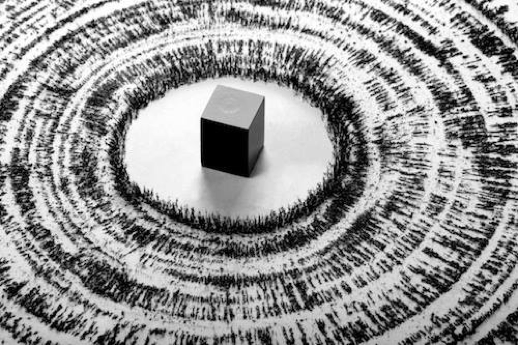
\includegraphics[width=1\textwidth]{imagenes/imagenes10/ExperientiaDocet01.png}
	\end{figure}

La palabra “campo” se usa de maneras muy diversas y puede llevar a confusión, por lo que merece la pena que nos detengamos un momento en ella. Empezaremos por el uso común de la palabra para ir introduciendo después, de forma paulatina sus significados en física (efectivamente, sigue teniendo más de un sentido incluso en física). Este pequeño ejercicio nos permite de paso recordar que la mayoría de los términos usados en física son adaptaciones de palabras usadas en la vida ordinaria, pero a las que se dota de significados específicos. Otros ejemplos son velocidad, aceleración, fuerza, energía o trabajo. Comprender las diferencias entre el término físico y el común es fundamental para entender la física.

Uno de los usos comunes más frecuentes de la palabra campo (sobre todo en España) es “campo de juego” (en Iberoamérica quizás sea más frecuentemente “cancha”). Un campo de fútbol, por ejemplo, es un lugar donde dos equipos compiten según unas reglas que confinan la acción al área del campo. “Campo” en este caso significa región de interacción.

Otro uso habitual de la palabra campo se encuentra en el mundo de la geopolítica. En política internacional se habla de “esferas” o “campos” de influencia. Un campo de influencia política es también una región de interacción pero, a diferencia de un campo de juego, no posee una línea definida que marque sus límites. Unos países tienen más influencia que unos y menos que otros países. Por ello en el sentido político “campo” se refiere también a la cantidad de influencia, más en unos lugares y menos en otros. Además, en el caso político, el campo tiene una fuente, el país que ejerce la influencia.

Ya encontramos aquí similitudes con los conceptos de campo que se usan en física. Pero también con una diferencia importante. Para definir un campo en física tiene que ser posible asignar un valor numérico a la intensidad del campo en cada punto del campo. Esta parte del concepto de campo es más fácilmente entendible si consideramos dos situaciones de la vida cotidiana, primero en lenguaje ordinario y luego en términos físicos:

a) Voy andando por la acera, de noche, hacia una farola encendida. Veo que hay más luz conforme me acerco a ella.

b) Estoy quieto en una acera y oigo un coche que pasa de largo tocando la bocina de forma continua. Oigo que el sonido va aumentando de intensidad y luego disminuye.

	\begin{figure}[H]
	\centering
	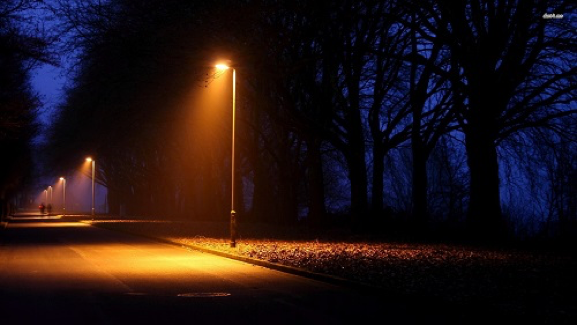
\includegraphics[width=1\textwidth]{imagenes/imagenes10/ExperientiaDocet02.png}
	\end{figure}

Podemos describir estas dos situaciones usando campos:

a) La farola está rodeada por un campo de iluminación. Cuanto más cerca estoy de ella, más fuerte es el campo de iluminación que registra mi ojo o el medidor de intensidad de luz (fotómetro) que llevo conmigo. A cada punto del espacio alrededor de la farola puedo asignar un número que representa la intensidad del campo de iluminación en ese lugar.

b) La bocina del coche está rodeada por un campo de sonido. Yo estoy quieto en mi marco de referencia (la acera). Conforme el coche pasa a mi lado con él se mueve un patrón de valores de campo con la misma velocidad que el coche. Esto es, el campo de sonido es estable pero se mueve con la bocina. En cualquier caso yo puedo asignar un número a cada punto del campo para representar la intensidad del sonido. Al principio el sonido es apenas audible conforme la parte más débil del campo me alcanza. A partir de ahí comienza a subir la intensidad del campo y el sonido parece más fuerte. Finalmente, la intensidad disminuye al alejarse el campo de sonido y su fuente (la bocina).


Démonos cuenta de que en los campos que hemos considerado ambos están producidos por una sola fuente. En a) la fuente es una farola estacionaria y en b) es una bocina en movimiento. En ambos casos la intensidad del campo aumenta gradualmente conforme mi distancia a la fuente disminuye. Asociamos un valor numérico a cada punto del campo: estamos ante ejemplos de campos escalares sencillos. El concepto de dirección no aparece asociado al valor del campo en cada punto.

Entre los dos mapas que encuentras a continuación hay una diferencia significativa entre los campos representados en ambos. En el primero, en el que se representa la presión atmosférica y en el que las líneas (isobaras) unen puntos con igual valor de la presión, un solo número (una cantidad escalar) da el valor del campo en cada punto. Pero en el segundo, en el campo de la velocidad del viento, el valor del campo viene dado tanto por un valor numérico (llamado magnitud, representado por la escala de colores) y una dirección (representada por las flechas); la combinación de magnitud y dirección es lo que constituye un vector y por ello el campo de llama vectorial.
	
	
	\begin{multicols}{2}
	\begin{figure}[H]
	\centering
	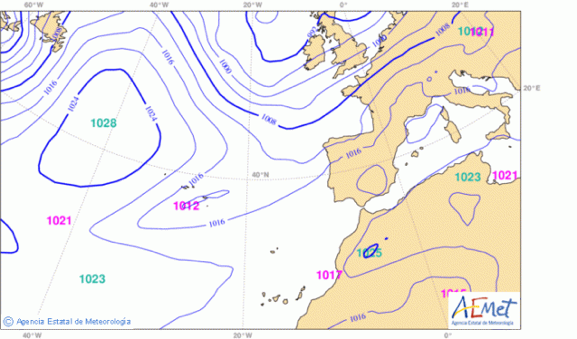
\includegraphics[width=0.5\textwidth]{imagenes/imagenes10/ExperientiaDocet03.png}
	\end{figure}
	Presión atmosférica
	\begin{figure}[H]
	\centering
	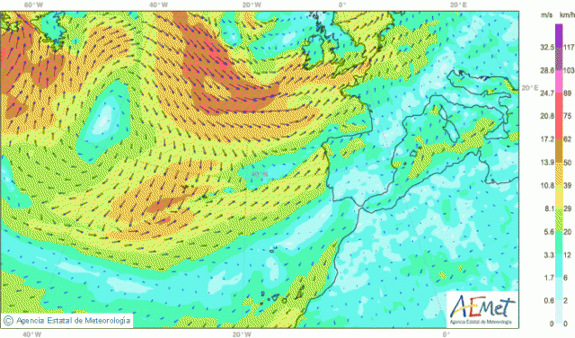
\includegraphics[width=0.5\textwidth]{imagenes/imagenes10/ExperientiaDocet04.png}
	\end{figure}
	Velocidad del viento	
	\end{multicols}





Finalmente, los físicos usan la palabra “campo” en tres sentidos adicionales a la definición de campo que hemos visto:

1) el valor del campo en un punto del espacio;

2) el conjunto de todos los valores en todos los puntos del espacio donde existe el campo;

3) la región del espacio en las que el campo toma valores distintos de cero.

Habitualmente, el contexto deja claro a cual de los conceptos de campo nos estamos refiriendo.

\vspace{4mm} \textcolor{gris}{Sobre el autor: \emph {César Tomé López es divulgador científico y editor de Mapping Ignorance.}}





%\begin{proofw}\renewcommand{\qedsymbol}{$\diamond$}
% \overrightarrow { v' } 





	
